\chapter{Introduction}\label{CHAP1}

%%%%%%%%%%%%%%%%%%%%%%%%%%%%%%%%%%%%%%%%%%%%%%%%%%%%%%%%%%%%%%%%%%%%%%%%%%%%
%  Motivation
%%%%%%%%%%%%%%%%%%%%%%%%%%%%%%%%%%%%%%%%%%%%%%%%%%%%%%%%%%%%%%%%%%%%%%%%%%%%
\section{Motivation}\label{CHAP1_1}
% 1 Constellations, % 2 Collision Avoidance - recent Starlink, OneWeb
The proliferation of satellites and spacecraft launched in the last decade has accelerated the need for better enhanced situational awareness of the space asset's surroundings and greater autonomy operating in the very congested Low Earth Orbit (LEO), Middle-Earth Orbit (MEO) and Geosynchronous Orbit (GSO) space environment. The recent April 2021 smallsat\footnotemark{} market report conducted by Eurconsult (Fig. \ref{fig:smallSatMarket}) estimates 13,910 smallsats (defined as $<$500 kg) will be launched in the next decade, a significant 370 \% increase from the previous decade. This growth is driven by commercial mega constellation communication LEO satellites, accounting for 38 \% of all smallsats. A Google search survey of the planned number of constellations is summarized in Table \ref{table:constellation}. 

%---------------------------------------------------------------------------
\begin{figure}[ht]
    \centering
    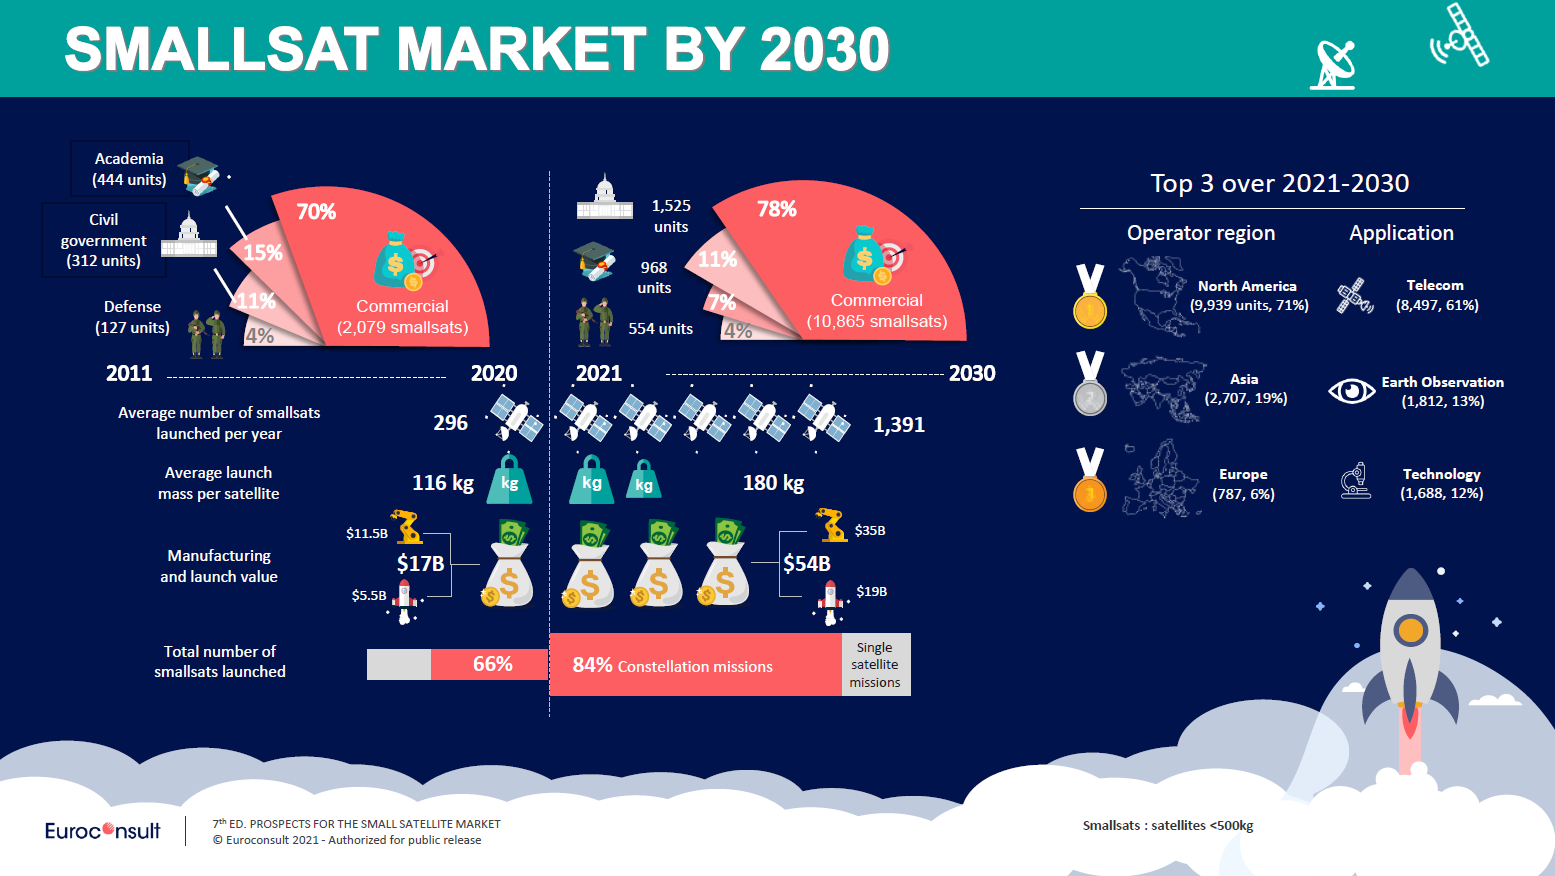
\includegraphics[width=1\textwidth]{Figures/EuroconsultSmallSatMarketBy2030.PNG}
    \caption{Small Satellite Market Survey 2021 \cite{euroConsult21}}
    \label{fig:smallSatMarket}
\end{figure}

%---------------------------------------------------------------------------
\begin{table}[!ht]
    \centering
    \caption{Current and planned Mega-Constelllations}
    \label{table:constellation}
    \resizebox{\textwidth}{!} {%
    \begin{tabular}{||c c c c||} 
    \hline
    Constellation & Organization & No. of Sats (full service est.) & altitude \\ [0.5ex] 
    \hline\hline
    Starlink\footnotemark{} & SpaceX &  42,000 & 580 km \\ 
    \hline
    OneWeb\footnotemark{} & OneWeb & 6372 & 1,200 km \\
    \hline
    Lightband\footnotemark{} & Telesat & 298 & 1,325 km \\
    \hline
    Kuiper\footnotemark{} & Amazon Kuiper LLC & 3,236 & 590 km, 610 km, 630 km \\
    \hline
    GuoWang\footnotemark{} & CASC & 12,992 & 508 km, 590 km, 600 km, 1,145 km \\ [1ex]
    \hline
    \end{tabular}
    }
\end{table}

\footnotetext[1]{Satellite mass definitions used in this dissertation are defined as follows: Cubesats $<$ 50 kg, Microsats 51 - 150 kg, Smallsats 151 - 500 kg} 
\addtocounter{footnote}{-4}
\footnotetext{\href{https://en.wikipedia.org/wiki/Starlink}{Wikipedia, "Starlink", May 5, 2021 [Online]}}
\addtocounter{footnote}{1}
\footnotetext{\href{https://en.wikipedia.org/wiki/OneWeb}{Wikipedia, "OneWeb", May 5, 2021 [Online]}}
\addtocounter{footnote}{1}
\footnotetext{\href{https://www.telesat.com/wp-content/uploads/2020/08/Telesat-Lightspeed-Defence.pdf}{Telesat, "Telesat LighSpeed", May 5, 2021 [Online]}}
\addtocounter{footnote}{1}
\footnotetext{\href{https://en.wikipedia.org/wiki/Kuiper_Systems}{Wikipedia, "Kuiper System", May 5, 2021 [Online]}}
\addtocounter{footnote}{1}
\footnotetext{\href{https://spacenews.com/china-is-developing-plans-for-a-13000-satellite-communications\-megaconstellation/}{Jones, A., "China is developing plans for a 13,000-satellite megaconstellation", SpaceNews, Apr. 21, 2021 [Online]}}
\addtocounter{footnote}{1}
\footnotetext{\href{https://spacenews.com/china-is-developing-plans-for-a-13000-satellite-communications\-megaconstellation/}{Liberatore, S., "SpaceX, OneWeb Satellites Come Within 190 Feet Of Each Other In Orbit", Space News, Apr. 9, 2021 [Online]}}

As of April 2021, Starlink has 1,383 satellites in orbit at 550 km altitude and OneWeb has 146 satellites in orbit 1,200 km altitude. On April 4th 2021, the StarLink and OneWeb satellites came within 190 feet of each other, triggering several red alerts from the US Space Force 18th Space Control Squadron to issue a warning to OneWeb who immediately maneuvered their 36 satellites launched recently on March 30th, 2021\footnotemark{}. This event exemplifies, 1) the very real danger of space asset collision leading to the Kessler Syndrome (ablation cascading) \cite{KesslerSyndrome78} without even accounting for the existing space debris that active space assets will have to avoid, and 2) the dependency of ground tracking measurements, data triage and human-in-the-loop decision making process space situational awareness. Clearly, the co-existence of these mega-constellations with existing and planned future space assets is extremely fragile.

%---------------------------------------------------------------------------
% DND, DRDC, Dark Arts
This concern has been been elevated in relevance within Canada's Department of National Defense (DND) to issue two Request for Information (RFI) in 2019 for the Surveillance of Space Ground (GBO) and Space based observation (SBO) \cite{dndRfi19a} - \cite{dndRfi19b}, a follow-on to the successful Sapphire microsatellite mission under the DND's Space Domain Awareness (SDA) Secure, Strong, Engaged Program. Sapphire is the first dedicated space-based RSO surveillance asset and has become an integral to the Canadian Space Operations Center's (CANSpOC) contribution to the Combined Space Ops (CSpOC) with US SPACECOM,  UK Space Operation Center (UK SpOC) and the Australian Space Operations Center (AUS SpOC). Concurrently, Defence Research and Development Canada (DRDC) issued an Innovation Call for Proposal  \cite{drdcCall19} for a space-based autonomous close-loop tracking Resident Space Object (RSO) surveillance microsatellite, a follow-on to NEOSat, under Space Technology Challenge No.15. One of five key technologies to be demonstrated is detection of RSOs within close orbital proximity of the microsatellite, reflecting the emphasis of an onboard space situational awareness (SSA). Such a capability would be essential in detecting hostile satellites in a space-to-space space-weapon framework as discussed in the "Protecting Space Systems from Counterspace Weapons" report by the Center for Strategic \& International studies \cite{darkArts21}. In addition, the listed active space-based defense strategy such as physically capturing the threatening object to disable or move it, which can also double as an inspector an on-orbit servicing satellite, requires a very robust onboard SSA coupled to a close proximity control system. A similar onboard SSA system would greatly benefit commercial mega-constellation space assets, providing greater ability to be self-aware of it's surrounding and to react autonomously in real-time.

% 4 GSO In-Orbit Servicing MEV-1.
In the case of an on-orbit servicing (OOS) system, previous concept studies and designs in last two decades \cite{tatschOss06,floresabadReviewSpaceRobotics20141} has finaly been realized by Northrop Grumman's Mission Extension Vehicle (MEV-1) \cite{mev121}. MEV-1 successfully rendezvoused with, refueled and and re-positioned the IntelSat 901 to GEO service in February 25th, 2020.  Northrop Grumman did it again with MEV-2, repeating the feat with Intelsat 10-02 on April 13th 2021\footnotemark[8]{}.
\footnotetext{\href{https://spacenews.com/mev-2-servicer-successfully-docks-to-live-intelsat-satellite/}{Rainbow, J., "MEV-2 servicer successfully docks to live Intelsat satellite", Space News, Apr. 12, 2021 [Online]}}
However, as highlighted by Harrison et al.\cite{darkArts21}, the host satellites are cooperative, similar to Space-X's Dragon capsule, Soyuz or ATV cargo spacecraft approaching and docking with the International Space Station (ISS) using proximity cameras in the visible-infrared spectrum and Light Detection and Ranging sensors (LiDARs) assisted by known physical markers \cite{OpromollaPose17}. These cooperative proximity sensing greatly improves the accuracy of rendezvous and docking operations. The distinguishing feature of a military defensive capability however, is the ability to conduct remote proximity and docking operations with an uncooperative or uncontrolled space object.These operations are extremely challenging when there is no consent from the host satellite or the satellite is lost, i.e. the target space object could make unexpected movements, may be tumbling, or may react unexpectedly to the docking if its automatic position and attitude control system remains engaged. 

 % 5 Debris Removal, Astroscale
The field of Active Debris Removal (ADR) missions architectures and technology development only came into prominence in 2007 when A Russian Briz-M booster stage exploded in orbit over South Australia generating 1,000 fragments \cite{bonnalAdr13}. Due to the nature of the uncooperative debris, vision technologies mentioned previously for 'dark' satellites will be limited in accuracy due to the various derbis size and characteristics \cite{limAdrVision13}.  The challenge of approaching a non-cooperative target has not deterred Astroscale's commercial vision to removed space debris. The Elsa-D microsatellite debris removal demonstrator, affectionately known as a "space sweeper", recently launched on March 22nd, 2021 \footnotemark{}, will move towards a test debris using GPS information, estimate its exact position and analyze its motion with (undisclosed) sensors and then will determine a path to approach the space junk before latching onto it using a magnetic docking plate. The space junk will be released before capturing another derbis and repeating the capture maneuver\cite{elsaD19}.
\footnotetext{\href{https://asia.nikkei.com/Business/Aerospace-Defense/Japan-s-Astroscale-launches-space-debris-removal-satellite}{Obe, M, "Japan's Astroscale launches space debris-removal satellite", Nikkei Asia, Mar. 22, 2021 [Online]}}

% 6 Lunar Gateway
Moving beyond GSO, NASA’s ambitious Artemis Program to land the first woman and the next man on the Lunar south pole by 2024 \cite{nasaArtermis20} and the goal to establish a Lunar gateway \cite{winternitzGpsLunarGateway19} by 2026 will see an increase of space traffic in Cis-Lunar space. A spacecraft bound for the Lunar Gateway will be guided by absolute trajectory knowledge with a certain level of accuracy, typically in the 100ths of km range. The GPS navigation experiment onboard the four Magnetospheric Multi-Scale (MMS) spacecraft had demonstrated the ability to receive GPS signals at extremely high altitudes, 4.6 times higher than GSO \cite{winternitzGpsLunarGateway19} and feasibility studies by Capuano et al.,  \cite{capuanoGpsLunarNav16} and Delépaut et. al, \cite{DelepautGpsLunarNav16} has proven that receiving GPS L1 signal is feasible within the moon transfer orbit. As the spacecraft approaches the Gateway to within meters in range to docking, precise relative position and orientation knowledge of the spacecraft is crucial in ensuring the spacecraft matches the the orientation of the Gateway. Although cooperative in nature; the approximately 400,000 km distance to be travelled  and line-of-sight of the deep-space communication link will result in delayed and limited command and telemetry operations. Hence the need for robust autonomous situational awareness and proximity system is imperative. This operational challenge is reinforced by the joint Canadian Space Agency/ MDA information session for the Lunar Gateway’s Canadarm3 \footnotemark{} that identified technical gaps for the robotic arm, i.e., situational awareness, proximity sensing, collision avoidance, supervise autonomy, and the need for AI autonomy.
\footnotetext{\href{https://mda.space/en/mda-launchpad/}{Canadian Space Agency-MDA, "Canadian Space Agency Canadarm3 information session", Jan 14, 2021}}

% 7 Asteroids
The field of asteroid exploration combines the two challenges of an uncooperative target and delayed communication link to Earth as evident in both the HAYABUSA (MUSE-C) mission \cite{Kobayasi3DofPoseAsteroid15} and OSIRIS-REX \cite{leonarOsirusRex19}. Both spacecraft missions successfully returned asteroid samples relied heavily on visual and lidar images for relative position and orientation of the asteroid to the spacecraft with careful, and complex, navigation and proximity events to "landing and descent" of the Asteroid sample tool. In the case of OSIRIS-REX, an onboard optical navigation system that compares observed images to a set of asteroid terrain models which are rendered in real-time from a catalog stored in memory on the flight computer, and onboard knowledge of the spacecraft state is then updated by a Kalman filter using the measured residuals between the rendered reference images and the actual observed images \cite{lorenzOsirusRexAutoNav}.      

% 7 Formation Flying
Situational awareness and proximity sensing are also critical in satellite formation flying (FF). Measurement missions that require precise baseline separations such as synthetic aperture radar, gravimetry, and deep-space observation, are significantly enhanced when the measurement baseline is distributed to individual space assets \cite{frasierAdaptiveKF18}. These assets will need to know their relative position and orientation with respect to each other, sometimes down to the cm range to ensure tight formation flying. Similar to operations in Cis-lunar space, future deep-space science missions like LISA located at 0.35 AU from Earth \cite{amatoFormationFlying19} will encounter similar communication delays with even more stringent attitude requirements. Hence an autonomous and adaptive relative navigation and attitude estimator ensures intelligent and timely responses for safe operations in the absence of human decision making processes.   

The underlining denominator for all scenarios outlined for a spacecraft with respect to another, is a close-loop event that can be synthesized into three processes; 1) situational or proximity awareness (sense), 2) task planning (reasoning or control); and 3) task execution (actuation). Within situational or proximity awareness, the term pose estimation is frequently used. Specifically, pose represents the combination of the \textit{position} and \textit{orientation} of an object \textit{relative} to another object, or reference point within a defined coordinate system \cite{PrezVillar2017SpacecraftPE}.  Pose estimation is the specific task of determining the pose of an object using proximity sensors. The pose estimation are distinct for each scenario that the spacecraft needs to operate, which can be summarized as follows:
\begin{enumerate}
    \item Cooperative and non-cooperative collision avoidance; 
    \item Cooperative and non-cooperative rendezvous; 
    \item Cooperative contact and non-cooperative contact; and
    \item Formation Flying.
\end{enumerate}

The pose estimator designed for one environment is not necessarily applicable to another. Hence, the motivation of this research is to explore and develop a dynamic, adaptive and autonomous space asset pose estimator that is agnostic to any space scenario.

%%%%%%%%%%%%%%%%%%%%%%%%%%%%%%%%%%%%%%%%%%%%%%%%%%%%%%%%%%%%%%%%%%%%%%%%%%%%
%  Problem Statement
%%%%%%%%%%%%%%%%%%%%%%%%%%%%%%%%%%%%%%%%%%%%%%%%%%%%%%%%%%%%%%%%%%%%%%%%%%%%
\section{Problem Statement}\label{CHAP1_2}

Pose sensors mounted on a space asset provide physical measurements that are mapped to the position and orientation of the space asset's body frame relative to another frame, whether it is a Earth centered fixed inertial (ECI) or another spacecraft body reference frame \cite{PrezVillar2017SpacecraftPE}. The scenario discussed in the previous section is more suitably labeled as relative pose estimation using different definitions of dynamic and kinematic equations that define the relation between the two spacecraft body frames \cite{OpromollaPose17}.  In generally; the process to determine the kinematic and dynamic position and orientation relationship can be establish using there main approaches \cite{landisMarkleyFundamentalsOfADCSSpacecraft15}:
\begin{enumerate}
    \item deterministic (determination);
    \item probabilistic (estimation); and   
    \item combination of deterministic and probabilistic approaches. 
\end{enumerate}

Note the term determination is broadly used in literature to include estimation. There is, however, a clear distinction where determination is solely a deterministic algebraic vector process, whereas estimation is an indirect vector modelling process \cite{Dhahbane2021AttitudeDA}. This dissertation will use the broad definition of determination except when a clear distinction is required. 

Both the deterministic and probabilistic approaches are reliant on sensor performances that depend on the physical principal of the system and quality of the components. For example, visual cameras are dictated by the physical optics (aperture size, focal length, lenses curvature and surface finish), detectors (pitch length, radiometric sensitivity) and read-out electronics (integration time, analogue digital conversion, clock frequency). For a Global Navigation Satellite System (GNSS) receiver mounted on both space assets to determine relative position, i.e. differential GNSS techniques, the position telemetry depend on the performance of the GNSS antenna gain, temperature and line noise, and electronic  acquisition, tracking and FPGA navigation processing. These sensors are cost sensitive, where better performance detectors and electronics will cost higher \cite{hashim2021attitude}. The inherent sensor noise that exist decreases pose determination accuracy. Hence a deterministic pose approach is shackled to the sensor noise unless algorithm data processing and filtering are employed to improve accuracy\cite{OpromollaPose17}.

A probabilistic approach uses probability techniques to minimize the difference between the state models (the estimate) to the actual sensor measurements, i.e. a cost function regression exercise. The ubiquitous Kalman filter (KF) used in  aerospace guidance, navigation, attitude and orbit estimation is simply a weighted recursive least square coupled to a state space dynamic model 'propelled' by propagating and correcting the process and measurement noise variance \cite{franklinDigitalControl97}. The recursive framework is important for real-time implementation onboard the spacecraft, versus batch post processing and the statistical approach assumes a normal Gaussian distribution for both the process and measurement noise - which are idealistic in reality. For pose estimation, the state dynamics are non-linear. Similarly the pose sensor physical measurements mapped to the estimated states can be non-linear, which violates the linear assumption of the Kalman Filter. Hence a local linearization of the state transition matrix and the measurement matrix are required at each time-step. This approach is sup-optimal as the state transition matrix for example relies on a Taylor series expansion and the idealistic Gaussian noises. In most implementation cases; the Taylor series is truncated and only the first two dominant terms are considered but the Gaussian noises are still assumed \cite{franklinDigitalControl97,cavenagoEkfHighOrder19}. This version is called the Extended Kalman filter (EKF) and serves well in most benign orbit position and orientation (attitude) estimation. The dynamic range of the space asset operating in the three broad scenarios described in Section \ref{CHAP1_1} from km to m in range however, produces a time variant noise that in most formulations of the EKF are considered static in nature. This limits the utilization of the EKF pose estimation to within well defined noise envelopes i.e., a near range environment. Unlike co-operative targets that would provide active markers \cite{OpromollaPose17}, space assets approaching non-cooperative targets are solely dependant on the pose sensor performance. Ideally, pose estimation should be inclusive of both the near range and far range pose sensor measurement environment i.e., as the spacecraft approaches from a few kilometers to within meters or centimeters for direct contact. This essentially improves situational awareness during all phases of the space asset approaching the target, improving task planning and optimizing task execution i.e., reducing delta-V, the propellant required to complete the entire closed-loop process for estimating the proximity of other space assets, rendezvous and docking, and formation flying.


%%%%%%%%%%%%%%%%%%%%%%%%%%%%%%%%%%%%%%%%%%%%%%%%%%%%%%%%%%%%%%%%%%%%%%%%%%%%
%  Previous Work
%%%%%%%%%%%%%%%%%%%%%%%%%%%%%%%%%%%%%%%%%%%%%%%%%%%%%%%%%%%%%%%%%%%%%%%%%%%%
\section{Previous Work}\label{CHAP1_3}
The earliest pose estimation studies, or in more generic terms, relative navigation, stems from the early Gemini missions \cite{chamberlinGemini64} which led to the Apollo missions \cite{youngApollo70} for orbital rendezvous, docking and control (RODC). This is essentially cooperative rendezvous and contact between two spacecrafts as discussed in Section \ref{CHAP1_1}. These early RODC missions rely on Radio-Frequency (RF) antennas installed on-board both the chaser and the target. The RF frequencies were exploited to obtain range, range-rate, Line-of-sight (LOS) angles and relative attitude parameters within several kilometers of precision \cite{fehse_2003, woffidenRez07}. RODC in general consists of  several phases that can be generalized in  Figure \ref{fig:rendezvousPhase}. During the phasing period, absolute navigation is in operations and as the chaser enters the close-range rendezvous phase, relative navigation is initiated. The homing and closing sub-phases ranges in kilometers and as the spacecraft enters the final approach phase to the target, relative position, velocity, attitude and angular rate information are required by the chaser to ensure a  straight light approach to docking. 

These legacy on-board RF systems used in RODC, however, are massive and have now been superseded with on-board Global Positioning System (GPS) receivers used spacecraft missions such as GRACE \cite{tancrediGraceOnboard10}, Tandem-X \cite{jaggiTandemX12} and PRISMA \cite{dAmicoPrisma11}. These relative positions used differential GPS techniques post-processed or performed on-board. For post processing, GRACE achieved a relative position precision of 1.56 mm 3D standard deviation \cite{kroedGracePostProcess06}, while Tandem-X achieved 1 mm 3D standard deviation \cite{jaggiTandemX12}. For on-board processing however, the near real-time relative distance precision for GRACE was within 4.2 cm 3D RMS \cite{tancrediGraceOnboard10} and 5.0 cm 3D RMS for PRISMA \cite{dAmicoPrisma11}. GRACE and it's follow-on mission Grace II \cite{sheadGrace2Inter12} and PRISMA have demonstrated relative position accuracy lower than centimeters using dedicated inter-satellite ranging (ISR) systems as summarized in Table \ref{table:isrMissionAccuracy}. These missions are not RODC and in fact are true FF operational missions. 
%---------------------------------------------------------------------------
\begin{figure}[ht]
    \centering
    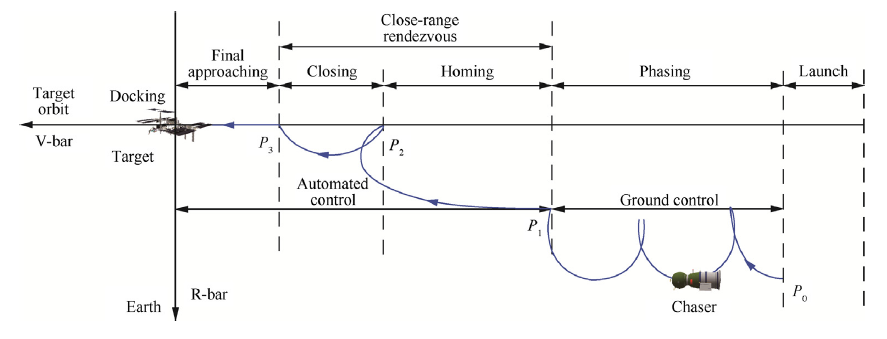
\includegraphics[width=1\textwidth]{Figures/LuoSurveyOfRelativeNavigation.PNG}
    \caption{Generic spacecraft rendezvous and docking phases \cite{luoSurvey13}}
    \label{fig:rendezvousPhase}
\end{figure}
%---------------------------------------------------------------------------

%---------------------------------------------------------------------------
\begin{table}[!ht]
    \centering
    \caption{Inter-satellite ranging (ISR) systems performance for  LEO FF missions}
    \label{table:isrMissionAccuracy}
    \resizebox{\textwidth}{!} {%
    
    \begin{tabular}{||c c c ||} 
    \hline
    Mission & ISL type & Relative Position Accuracy \\ [0.5ex] 
    \hline
    GRACE\cite{tapleyGraceIsr04} & microwave ranging &  10 \mu m \\ 
    \hline
    GRACE-II\cite{sheadGrace2Inter12} & microwave ranging \& laser interferometry & 50 nm \\
    \hline
    PRISMA\cite{monterbruckPrismaIsr08} & microwave ranging \& vision-based sensor & 0.1 m \\
    \hline
    \end{tabular}
    
    }
\end{table}

The relative pose estimation for these RODC and FF missions can be better categorized. Luo et al. \cite{luoSurvey13} divided navigation sensors into relative and absolute sensors. Absolute navigation sensors determines the spacecraft position and attitude in the inertial frame using navigation equipment, inertial measurement units and optical attitude sensors. Examples include RF ranging with a tracking ground terminal, on-board GPS position, velocity, time (PVT) measurements for position and star trackers for attitude. Relative sensors on the other hand determines the chaser's position, velocity, attitude and angular rate with respect to the target using optical, radio, laser or laser interferometry \cite{yangInterSatelliteGrace13}. Examples includes microwave radars and lidars. 
Oppromila et al.\cite{OpromollaPose17}, provided an excellent taxonomy of these electro-optical sensors used for relative pose estimation as shown in Figure \ref{fig:taxonomyEo}. 
%---------------------------------------------------------------------------
\begin{figure}[ht]
    \centering
    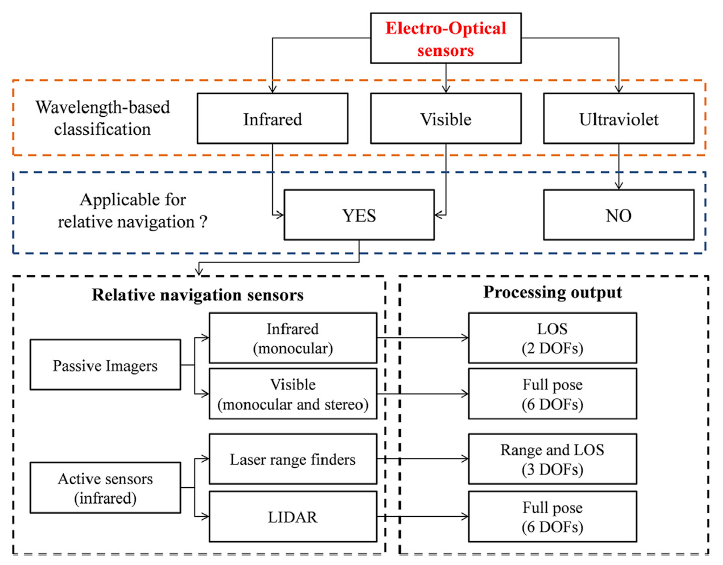
\includegraphics[width=1\textwidth]{Figures/OppromolaTaxanomyPoseSensors.PNG}
    \caption{Taxanomy of Electo-Optical relative pose sensors \cite{OpromollaPose17}}
    \label{fig:taxonomyEo}
\end{figure}
%---------------------------------------------------------------------------
The determination of the relative pose states are either deterministic instantaneous from sensor outputs or the filtered historic outputs of these measurements, i.e., estimation as mentioned in Section \ref{CHAP1_2}. For the former, relative distance and velocity are determined using either RF, GPS, laser ranging or interferometry as implemented by CRACE, Tandem-X and PRISMA. The distance, velocity and attitude information can also be obtained directly based on geometric extraction of feature points monocular visual system images \cite{aghiliPoseVision10, leiPoseSlam19, sharmePoseNonC17a, ShijieMono10}. PRISMA in particular utilized both microwave ranging and vision-based sensors \cite{monterbruckPrismaIsr08}.

For the pose estimation using models and probabilistic techniques, the Extended Kalman filter (EKF) is the most widely used filter algorithm for relative navigation \cite{dAmicoPrisma11,karlgaardAdaptiveEkf11}. These EKF utilizes either Clohessy–Whiltshire (C–W) equations \cite{CW} for circular orbits or Tschauner and Hempel (T-H) equations \cite{Tschauner65} for elliptical orbits in the state model and has shown to provide a wider operational range and better standard deviations for pose accuracy compared to deterministic techniques. Indeed, PRISMA's  8 state EKF (3 for relative psotion, 3 for relative velocity and 2 for bearing angle bias) reported a relative centimeter accuracies from  10 km ranges down to 100 m, with long period proximity operations reported at 1 am standard deviation \cite{bodinPrisma12} using an EKF and GPS measurement updates. The fusion Close Range camera produced a bearing (attitude) accuracy between the MANGO-TANGO spacecraft less than 0.1\textdegree at distances of 20 meters. The robustness of the EKF has been applied for numerous other spacecraft, including the Can-X4 and Can-X5 satellites \cite{boninCanX} and has proven well for RODC, OOS and FF scenarios where the target spacecraft in all cases are cooperative. But what of uncooperative targets?

%%%%%%%%%%%%%%%%%%
% Uncooperative and EKF-SLAM
%%%%%%%%%%%%%%%%%%
\subsection{Unccooperative pose estimation}\label{CHAP1_3_0}
Uncooperative pose estimation poses extreme challenges where the chaser pose sensor must decipher its relative pose to the target with no additional assistance. Sharma et. al managed to deal with non-cooperative target images using a monocular vision, reduced  dynamics pose multiplicative EKF (MEKF) based on D'Amico's Relative Orbital Elements (ROE) \cite{dAmicoPhdthesis} and image processing fusing weak gradient elimination technique with teh Sobel operator followed by Hough transform to detect both small and large features of the target spacecraft \cite{sharmePoseNonC17a}. Comparisons with the numerically simulated ground truth of the three relative trajectory test cases show the accuracy of the pose estimates to be at the level of 0.4376 \textdegree (3D rms error) and 0.0755 m when initialized with a pose solution with a relative position error of 0.1732 m (3D rms) and a relative attitude
error of 10.100 \textdegree (3D rms). The filter also relies on the pseudo-measurements of a normal vector generated from the pixel locations of the target spacecraft’s edges, thereby making the filter robust to the detection of partial edges in the image.The navigation filter’s robustness is also exhibited by undergoing stress-test with varying levels of pose initialization errors, measurement noise, and measurement update intervals. With an increase of the measurement noise of the pixel locations, the accuracy only worsened for the relative position in the bore-sight direction. The navigation filter is shown to provide precise and accurate pose estimates with an initial position error of up to 0.8 m.  

An alternate uncooperative pose estimation approach using the EKF is the Simultaneous Localization and Mapping (SLAM)-EKF \cite{sonnenburgEKFSlam010339} inherited from the robotics community. SLAM algorithms use characteristic points in the 3D environment, so called landmarks, to navigate relative to a mobile robot. Sonnenburg et, al defined the relative position of the target spacecraft as a landmark (the map). The relative position of the 'static' chaser (localization) are computed simultaneously by using the EKF using the C-W equations and monocular images, where the unobservability of the target features can be dealt by using an inverse depth parameritization method \cite{civeraInverseDepthParameritization08}. Oppromo et. al also surveyed other EKF-SLAM implementation using multiple iterated extended Kalman filters (IEKFs) and replacing the monocular sensor with stero vision \cite{OpromollaPose17}. However, they concluded that there are still open issues i.e., the capabilities and limitations of the EO sensors\footnotemark{} and the process model equations are obtained with a low fidelity relative motion  models for both rotational and transitional dynamics in the process equation. Nevertheless, the popularity of the EKF for pose estimation for cooperative and uncooperative targets is never doubted, hence the fundamentals and limitations of the EKF needs to be understood. 
\footnotetext{the papers surveyed only focuses on exclusively on the filtering and assumes 3D  features detected and tracked are inputs to the EKF}

%Kim et. al, \cite{kimPoseGyroYY} formulated the EKF using line-of-sight measurement with gyro measurements and an EKF.   

%during these phases are mostly done either by (1) angles-only relative measurement or (2) by image information. For the former; maximum measuring distances are limited to a few tens of kilometers for non-cooperative target rendezvous as distance measurements have large uncertainties. 
%For the latter, image measurements come in the form of charge-coupled device binocular or monocular vision measurements. Using monocular vision measurement will require the use of the Clohessy–Whiltshire (C–W) or Hill equations, for circular equations and Tschauner and Hempel (T-H) equations for elliptical orbits. 

%As expected the EKF has been the major filter algorithm used for rendezvous navigation. Particle filters was also employed in a few studies, although onboard implementation feasibility can be challenging given the computational recursion of the algorithm itself \cite{}. An adaptive method to automatically tune the Kalman filter by estimating measurement and processing noise co variance to improve the robustness of the filter for an elliptical rendezvous navigation problem had been investigated. 

\subsection{The Extended Kalman filter}\label{CHAP1_3_1}
The EKF has been the workhorse for many aerospace guidance, navigation and attitude determination systems since its inception in the 1960's. The EKF is the linearized version of the linear Kalman Filter (KF) formulated by Rudolph Kalman in his seminal paper "A New Approach to Linear Filtering and Prediction Problems" \cite{Klmn1960ANA}. The EKF was specifically formulated to resolve the measurement gaps encountered during the Apollo Service Module (and the attached Descent Module when outbound) during the 76 hrs Moon Transfer Orbit (MTO) trajectory. In particular; the EKF was used to determine when the Mid-Correction burns were required during transit. For history buffs, Grewal \cite{grewalKFHistory10} provides a very refreshing read on the beginnings of the EKF, its roots in spacecraft guidance and navigation, and the proliferation to GNSS and particular Inertial Navigation systems for terrestrial applications.  

The EKF is essentially a recursive process to estimate the a systems current state  from a set of measured observations. It involves finding the best estimate of the true system state using a dynamic model and measurement model that are both corrupted with random noise of known statistics \cite{landisMarkleyFundamentalsOfADCSSpacecraft15}, which are Gaussian and white. This is the foundation of the KF when in reality, they may not be \cite{franklinDigitalControl97}. As a side trivia, the KF is build-upon a weighted recursive Least Squares estimation (LSE) with an added dynamic component. Franklin aet. al provides an excellent step-by-step formulation of the EKF \cite{franklinDigitalControl97}. For other attitude specific EKFs, Landis-Markley et. al \cite{landisMarkleyFundamentalsOfADCSSpacecraft15} and De Ruiter et. al \cite{deRuiter2012spacecraft}, provides good context on the its implementation. 
 
The EKF are not without its limits. The EKF will still behave poorly and diverge if the system is either non-Gaussian or, even if the system is Gaussian, a large initial estimate will lead to divergence as well \cite{franklinDigitalControl97}. For example, the execution of an impulsive thrust results in state transitional acceleration that if not accounted for in the EKF dynamics, will lead to divergence of the estimated states in the corrector phase. To remedy this effect, adaptive filters have been introduced to automatically 'tune' the measurement and process noise covariances \cite{frasierAdaptiveKF18, woffidenRez07}. 

Frasier et al. developed a Maximum Likelihood Estimate Adaptive Extended Kalman Filter (AEKF-MLE) and Fuzzy Logic Adaptive Extended Kalman AEKF (FEKF) for FF spacecrafts. The MLE blends the state estimates and system identification by defining a set of parameters that influence a likelihood function based on the observed measurements and the filter state estimates (i.e., parameters such as the noise covariance matrices, dynamics state transition matrices, or the input mapping matrices), adaptations to these parameters within the Kalman filter can be updated in order to maximize the observed likelihood function. A novel addition to the MLE algorithm was made,through the inclusion of an intrinsic fixed-window smoother capable of harnessing information from past state estimates to improve the convergence of the MLE cost function. Fuzzy logic (FL) provides a method to include varying degrees of a value within the extremes defined by traditional logic and allows the human intuition of the EKF behaviour to be incorporated into the adaptation laws, thereby providing a flexible adaptation strategy, unlike the analytic AEKF-MLE. The FL uses performance metrics based on the theoretical and observed residual covariance matrices of the EKF. The resulting fuzzy rule base is defined such that updates to the noise covariance matrices will minimize the difference between the theoretical and observed covariances of the residuals. Both adaptive EKF methods proposed have shown to produce relative position and velocity estimates that were more accurate than estimates provided by the traditional EKF for a low-eccentricity near-Earth orbit formation (PRISMA), a highly-elliptical formation with large separations in kilometers (PROBA-3), and a low-Earth, moderately elliptical formation subjected to large measurement noises (PRISMA-like). Frasier et al tuned the FEKF fuzzy system based on the desired adaptation performance for each scenario, which is more flexible than the analytic AEKF-MLE. These algorithms however have not been augmented to include attitude estimation. In addition, the reported computational complexity for the analytic AEKF-MLE may not be easily implemented on-board implementation given the 12-state pose estimator. The FEKF is a likely a better candidate, but the \textit{a priori} step needed to manually 'tune' the FEKF for specific orbit scenarios limits the FEKF to be a truly autonomous pose estimator for various scenarios e.g., using the same FEKF parameters for RODC and FF. Finally, the performance of FEKF using the derived close-form relative position equations is unknown if thruster firings were to occur.

%Woffinden et al., developed an adaptive Hurber-based EKF to provide better covariance adaption to avoid filter divergence and the varying relative dyanmic elliptical FF \cite{woffidenRez07}.

An essential characteristic that most modern text gloss over for the EKF and KF is the fact that the estimator is fundamentally trying to minimize the cost function between the measured and modelled states. The KF is essentially a linear regression optimization problem which is the foundation of Artificial Intelligence (AI), or more specifically Machine Learning (ML) and Neural Networks (NN) solving linear regression problems. In a rudimentary sense, the ML, specifically the NN, is similar to a Fuzzy-Logic with an activation function to gate the output, but with the advantage of a lattice of interconnected weighted inputs. The very robust nature of NN may result in an implementation of a pose estimator that is autonomous and adaptable to the dynamic ranges of OOS, FF and RODC. 

\subsection{Pose estimation with Neural Networks}\label{CHAP1_3_2}
The evolution of Artificial Intelligence (AI), or more explicitly Machine Learning, has accelerated the transition of repetitive analytical task to be completed autonomously and within shorter time-frames. At the core of Machine Learning (ML) is the minimization of the cost function between a states or states that defines the model and the associated measurement or measurements, i.e. a linear regression or logistic regression process. Given that no dynamical models are required, unlike the KF / EKF, ML approaches, ML can prove an alternate approach to improve the pose estimation as defined previously. Neural-networks (NN) is a type of ML that mimics the human brain and expands on cost minimization process by modelling a network of state nodes, weighted and triage using an activation function (sometimes called a perceptron) at each layer to find the best possible outcome \cite{yangML21}. The work on Artificial Intelligence (AI), Machine Learning (ML) and its Neural Network (NN) subset as well as Deep Learning (DL) are continuously evolving at a daily rate. It would be a challenge task to present the evolution of this field of study and this literature review will only cover common applications of NN for pose estimation in the last decade.

The nascent spacecraft pose estimation using ML/NN have found to be limited to mostly vision based measurements. Sharma et al. \cite{sharmePoseNonCYYb} developed a Convolutional Neural Network (CNN) applied to the monocular images for pose estimation. Similarly, Prenca \cite{prencaDlPosePhotorealistic19} developed a probabilistic quaternion fitting pose estimator using Deep Learning. Mihai \cite{mihaiPoseAnn20} investigated the use of an onboard Artificial Neural Network (ANN) satellite orbit estimator with coefficients pre-trained using a 3-week training data set with mean errors less than a kilometer. The paper acknowledges that maintenance of these coefficient(s) is required, i.e. the need for periodic training to update the coefficients. To the best of the author's knowledge, the work by Forghani et al. \cite{ForghaniOrbitNN11},  is the only research comparing a satellite orbit estimation performance using an EKF only versus an on-line Neural Network only approach. His researched concluded that the NN provided a better orbit estimate compared to the EKF for the CHAMP satellite orbit parameters using an Earth tracking ranging station, including a simulated measurement outage. Both methods could cope well with ranging data outages, with the NN showing less estimation error than the EKF.

Nevertheless, terrestrial ground robotic research have explored the combination of EKF and NN for trajectory estimation. Bai's \cite{baiKf20} paper in particular has shown a improved trajectory estimation of a robotic rover traversing an elliptical race track using a tightly coupled trained on-board KF-ANN architecture. Unlike other terrestrial implementation research that performs EKF estimation that feeds into a ANN to improve performance or vice-versa, Bai's approach uses a two intermediate node ANN integrated into the KF predictor-corrector recursive loop. Node 1 minimizes the errors of the predicted KF where the results are then fed back into the KF measurement update. Node 2 then minimizes the errors after the KF measurement updated before sending the estimates back into the KF state prediction. The ANN uses a nonlinear aurotoregressive model with exogenous input (NARX) which basically takes the historic outputs and the associated historic inputs into the ANN, an effective reconstitute of the nonlinear system. The NARX model relates the current value of a time series to both past values of the same series; and current and past values of the driving (exogenous) series — that is, of the externally determined series that influences the series of interest \cite{menezesNarx20083335, baiCompund19}. In addition, the model contains which relates to the fact that knowledge of other terms will not enable the current value of the time series to be predicted exactly. In fact Forghani et al \cite{ForghaniOrbitNN11} was using a scaled down NARX NN to estimate the CHAMP orbit.     

ML however are not without its drawbacks. The probabilistic nature does not always guarantee the confidence of the approach in a space industry that is risk-adverse, particularly when human lives are at stake \cite{mcGovernMLSpaceLimits11, xuMLSpaceRelaibility2021107530}. The question that can be aske here is: similar previous work done for adaptive EKF, can the NN be used to adapt the measurement and process noise covariances without the limitations of the analytical AEKF-MLE or the FEKF? Based on the surveyed literature to date, none of these aforementioned studies involved the fusion of an EKF with a NN specifically for pose estimation. 
 
%%%%%%%%%%%%%%%%%%%%%%%%%%%%%%%%%%%%%%%%%%%%%%%%%%%%%%%%%%%%%%%%%%%%%%%%%%%%
%  Objectives
%%%%%%%%%%%%%%%%%%%%%%%%%%%%%%%%%%%%%%%%%%%%%%%%%%%%%%%%%%%%%%%%%%%%%%%%%%%%
\section{Thesis Objectives}\label{CHAP1_4}

The goal of this research is to develop a modular autonomous enhanced situational awareness technology for a spacecraft chaser to uncooperative target relative position and orientation for a dynamic range.

The primary objective of this thesis is to develop a near real-time EKF-NN for estimating the relative pose of a chaser spacecraft with respect to a tumbling uncooperative target spacecraft. Specifically, the EKF process and measurement noise covariances will be adapted using a Neural Network (NN), as function of the varying separation between both vehicles throughout a representative mission profile; from far-range approach to close-range rendezvous i.e., a 'tightly-coupled' EKF-NN similar to Bai's architecture \cite{baiKf20}. To the author's knowledge, this fusion has never been done before. The EKF-NN design, referred to as the Space Machine Attitude and oRbit inTelligence (SMART), assumes arbitrary computer vision algorithms will provide a rough pose measurement inputs (computer vision algorithms will not be the focus of this research). The expectation is that SMART will operate in any pose scenario, not be bounded by a pre-defined dynamic model and will only be constrained by the on-board processor performance, and sensor characteristics.  A Physical implementation on a Hardware-in-the-Loop (HIL) with a capable processor on an air-bearing chaser-target system will be conducted to verify the real-time performance limits. 

Given that this EKF-NN is intended to operate in any chaser-target range scenario, the ideal non-perturbed circular C-W equations \cite{CW} is ill-suited for the EKF state model. the precision of the C-W equation decreases as the relative distance increases, hence London \cite{londonSecondApproximateSol63} derived a widely used second-order relative dynamics equation, extending from the C-W equation, in the rectangular coordinate frame to improve the precision of the relative dynamic equations. This formulation however, is only limited to small orbit eccentricities. The T-H equation was formulated specifically for elliptical orbits, but researchers have not derived a simple closed-form solution, thus limiting its adoption in the field \cite{luoSurvey13}. Yamanaka et. al  derived a simpler equation using the true anomaly as the independent variable, which includes a non-zero total relative acceleration term. Not surprisingly, Frasier et. al's independently derived relative equations of motion \cite{frasierAdaptiveKF18} in the local vertical local horizontal frame (LVLH) of the chaser with respect to the target are exactly the same dynamic equations as Yamanaka et al.'s derivation. The difference lies in the frame of reference, where the later uses a target-orbit frame similar to a North-East-Down flight frame \cite{valladoAstrodynamics3rd}. Both Frasier's and Yamanaka's relative equations of motions handles highly eccentric orbits. D'Amico's relative orbital elements (ROE) \cite{dAmicoPhdthesis} is an alternate formulation.  
 
The relative attitude EKF state transition matrix will utilised the 1 x 4 unit quaternion and 1 x 3 relative angular velocity.  The 6 state relative position state transition matrix however will either use Yamanaka \footnotemark{} or  D'Amico's ROE. For the latter, this will be an exact implementation of Sharma and D'Armico's MEKF using the ROE \cite{sharmePoseNonC17a}. 

The process and measurement covriances will be updated using the NN NARX approach outlined in Bai et. al \cite{baiKf20} and Forghani et al. \cite{ForghaniOrbitNN11}. Note that an initial step is to implement a decoupled EKFand NN pose estimator to gauge the performance of each against the combined  EKF-NN.

Finally, if time permits, performance against Frasier et al's FEKF \cite{frasierAdaptiveKF18} updated with attitude estimation will be explored.
\footnotetext{The use of Yamanaka's formulation compared to Frasier's is simply a matter of the more common and easier relation to the orbital flight frame versus the LVLH frame, but will be finalized at a letter stage of this research}

%%%%%%%%%%%%%%%%%%%%%%%%%%%%%%%%%%%%%%%%%%%%%%%%%%%%%%%%%%%%%%%%%%%%%%%%%%%%
% Methodology
%%%%%%%%%%%%%%%%%%%%%%%%%%%%%%%%%%%%%%%%%%%%%%%%%%%%%%%%%%%%%%%%%%%%%%%%%%%%
\section{Methodology}\label{CHAP1_5}

%\begin{enumerate}
%    \item algorithm design in MATLAB (EKF only, EKF and NN, etc.)
%    \item simulation analysis with 3 scenarios (eg., docking with cooperative target, capture of %uncooperative target, approach with vision-only information),and
%    \item hardware-in-the-loop demonstration (describe the facility)
%\end{enumerate}

This research will follow subset of a space industrial ‘V’ requirements definition, analysis, development and verification in a software-based simulated environment followed by a hardware-in-the-loop (HIL) test bench. 

\begin{enumerate}
    \item This research is initiated with a literature review to define the motivation, problem statement, previous work and objectives. 
    \item A set of preliminary technical performance metrics (TPM) will be defined based on the literature review of previous work i.e. using the accuracies summarized in Table \ref{table:isrMissionAccuracy} as a reference. 
    \item A step-by-step  algorithm will be developed in MATLAB, (one state KF, linear regression, NN stand-alone and combined KF-NN) followed by the completed 6  state / 6 degrees of freedom (DOF) pose algorithm (EKF, EKF-NN). 
    \item A simplified relative orbit and attitude propagator in MATLAB will be developed to perform preliminary and optimization test the EKF-NN. 
    \item A complete Satellite Toolkit (STK Astrogator and EOIR module) rendezvous and docking scenarios, e.g. docking with a cooperative target, capture of uncooperative target) will be established to generate relative pose information to be used as the truth and to emulate a pose sensor inputs (baseline  vision-only information) to verify the EKF-NN in a higher fidelity simulated environment.
    \item The EKF-NN  will be verified using the STK  data and optimmized as applicable
    \item The next phase would be to deploy the algorithm using Matlabb's Autoco generator for Carleton University’s air-bearing chaser-target system that contains a NVIDIA AI capable processor with a basic camera, a Harware-in-the-Loop (HIL) system. The HIL's purpose is to test pose estimation and uncooperative target tracking in 3 DOF (2 DOF translation, 1 DOF rotation).
    \item The performance of this HIL will verify a real-time implementation of the EKF-NN algorithm in a real-world like terrestrial environment. Again, algorithm, optimization will be performed.
    \item Final analysis and results will be documented
\end{enumerate}

In parallel, the dissertation thesis chapters will be written in parallel per the schedule outlined in Section \ref{CHAP1_6}. Three journal papers will be developed for peer review and publication. The journals have yet to be identified. 

%%%%%%%%%%%%%%%%%%%%%%%%%%%%%%%%%%%%%%%%%%%%%%%%%%%%%%%%%%%%%%%%%%%%%%%%%%%%
% Schedule
%%%%%%%%%%%%%%%%%%%%%%%%%%%%%%%%%%%%%%%%%%%%%%%%%%%%%%%%%%%%%%%%%%%%%%%%%%%%
\section{Schedule}\label{CHAP1_6}
The preliminary research schedule will be aligned to seven (7) academic terms with three journal papers scheduled in term 3, 5 and 6 (TBD). The dissertation will be generated in term 1 and completed by term 7.
\begin{enumerate}
    \item Term 1 (Spring 21):  Perform literature review and generate chapter 1 of dissertation. Develop test algorithms.
    Deliverable: D1.1 Dissertation Chapter 1, D2.1: Test built

    \item Term 2 (Summer 21):  Develop preliminary EKF-NN. Development pose (6 DOF) simulator.  
    Deliverable: D1.2 Dissertation Chapter 2, D2.2 AttDet Algorithm built 

    \item Term 3 (Fall 21): Optimize EKF-NN. Development pose EO scenario.  
    Deliverable: D1.3 Dissertation Chapter 3, D2.3 AttDet Algorithm built, D3.3 Journal paper 1 draft
    
    \item Term 4 (Winter 22): Deploy the algorithm in HIL Testbench
    Deliverable: D1.4 Dissertation Chapter 3, D2.4 AttDet Algorithm built, D3.3 Journal paper 1 draft
    

    \item Term 5 (Spring 22): Review of data against TPM and optimize algorithm. Retest if needed. 
    Deliverable: D1.4 Dissertation Chapter 4, D2.5 AttDet Algorithm built, D3.5 Journal paper 1 final

    \item Term 6 (Summer 22): Complete Dissertation, update algorithm, generate journal paper 
    Deliverable: D1.5 Dissertation Chapter 5, D2.6 AttDet Algorithm built, D3.6 Journal paper 2 draft

    \item Term 7 (Fall 22): Complete Dissertation, update algorithm, generate journal paper
    Deliverable: D1.6 Dissertation Chapter 6, D2.7 AttDet Algorithm built, D3.7 Journal paper 2 final

    \item Term 8 (Winter 23): Complete Dissertation, update algorithm, generate journal paper
    Deliverable: D1.7 Dissertation Chapter 7, D3.8 Journal paper 3 draft and final

\end{enumerate}

%%%%%%%%%%%%%%%%%%%%%%%%%%%%%%%%%%%%%%%%%%%%%%%%%%%%%%%%%%%%%%%%%%%%%%%%%%%%
% Progress to Date
%%%%%%%%%%%%%%%%%%%%%%%%%%%%%%%%%%%%%%%%%%%%%%%%%%%%%%%%%%%%%%%%%%%%%%%%%%%%

\section{Progress to Date}\label{CHAP1_7}
\begin{enumerate}
    \item Term 1 (Spring 21):  Perform literature review and generate chapter 1 of dissertation. Develop test algorithms. DONE
    Deliverable: D1.1 Dissertation Chapter 1, D2.1: Test built

\end{enumerate}

%%%%%%%%%%%%%%%%%%%%%%%%%%%%%%%%%%%%%%%%%%%%%%%%%%%%%%%%%%%%%%%%%%%%%%%%%%%%
% Summary and Future Work
%%%%%%%%%%%%%%%%%%%%%%%%%%%%%%%%%%%%%%%%%%%%%%%%%%%%%%%%%%%%%%%%%%%%%%%%%%%%
\section{Summary and Future Work}\label{CHAP1_8}
Chapter 1 of the dissertation, i.e. literature review to define the motivation, problem statement, previous work and objectives have been defined. The schedule and deliverables have been drafted in this progress report. The next step is to develop the preliminary EKF-ANN and the reference attitude and body rate (6 DOF) simulator. Depending on the progress of the research, availability of this part-time student and Covid pandemic restricting HIL access, the three journal papers will be pull forward if favourable opportunities arise for the to-be-identified journals. 

%%%%%%%%%%%%%%%%%%%%%%%%%%%%%%%%%%%%%%%%%%%%%%%%%%%%%%%%%%%%%%%%%%%%%%%%%%%%
%  Thesis Organization
%%%%%%%%%%%%%%%%%%%%%%%%%%%%%%%%%%%%%%%%%%%%%%%%%%%%%%%%%%%%%%%%%%%%%%%%%%%%

%\section{Organization}\label{CHAP1_5}

%\lipsum